\documentclass[11pt]{article}

\setlength{\oddsidemargin}{-0.25 in}
\setlength{\evensidemargin}{-0.25 in}
\setlength{\topmargin}{-0.9 in}
\setlength{\textwidth}{7.0 in}
\setlength{\textheight}{9.0 in}
\setlength{\headsep}{0.75 in}
\setlength{\parindent}{0.3 in}
\setlength{\parskip}{0.1 in}
\usepackage{epsf}
\usepackage{pseudocode}
\usepackage{enumitem}
\usepackage{amsmath}
\usepackage{amssymb}
\usepackage{color}
\usepackage[normalem]{ulem}
\usepackage{graphicx}
\usepackage[export]{adjustbox}
\pagenumbering{arabic}
\def\O{\mathop{\smash{O}}\nolimits}
\def\o{\mathop{\smash{o}}\nolimits}
\newcommand{\e}{{\rm e}}
\newcommand{\R}{{\bf R}}
\newcommand{\Z}{{\bf Z}}

%% display solutions or not
\newif\ifsol
\soltrue % comment out to hide solutions

%% todo tracker -- overleaf v2 has better one it uses but will default to this if compiled on something that doesn't have built-in todo
\newcommand{\todo}[1]{\textbf{\textcolor{red}{#1}}}

\title{Section 8: Robot Motion Planning}
\author{CS 182 - Artificial Intelligence}
\date{}
\begin{document}
\maketitle

\renewcommand{\labelenumii}{\arabic{enumii}.}
\setlength{\parindent}{0pt}



\section{Definitions}

To make trajectory plans in robotics, we distinguish between two spaces:
\begin{itemize}
\item The {\bf{task space}} of a robot is the standard, Cartesian space in which it moves. It is usually defined by 3-dimensional (x, y, z) coordinates (but if one of the dimensions is irrelevant, such as for a Roomba, we can also define the task space by just (x, y)).
\item The {\bf{configuration space}} of a robot is the $n$-dimensional space of joint angles that fully defines the positioning of the robot. The number $n$ can be thought of as the number of degrees of freedom.
\end{itemize}

The relationship between a point in the task space and a point in the configuration space is determined by the structure and geometry of the robot. In the forward direction, {\bf{forward kinematics}} is the mapping of a robot configuration to an {\bf{end-effector}} (hand) position in task space. Conversely, {\bf{inverse kinematics}} maps a point in task space to a robot configuration. \\

Since the path-planning algorithms we discussed are based on random sampling, there are no deterministic guarantees of completeness and optimality that were discussed for search algorithms. Instead, we consider {\bf{probabilistic completeness}} and {\bf{probabilistic optimality}}, which ask whether algorithms are complete or optimal in the limit that the number of samples approaches infinity.


\section{Algorithms}

{\bf{Rapidly-exploring Random Tree (RRT):}} This algorithm accepts a start and goal location. To build a path, it iteratively: (1) samples states $s \in S$ until it finds one that is collision-free; (2) finds closest state $s_c \in T$; (3) extends $s_c$ toward $s$; (4) adds resulting state $s’$ to $T$; (5) repeats until $T$ contains a path from $s_0$ to $s_{goal}$. This algorithm is probabilistically complete, and searches for feasbile paths. A variant includes {\bf{goal-directed sampling}}, which augments the sampling step (1). Instead of just sampling randomly, we sample the goal with a (small) probability $p$. This makes it more likely that the tree actually reaches the goal, rather than waiting until it "stumbles" into it.\\

{\bf{Bi-directional RRT:}} This a variant on RRT which grows two trees -- one starting from the start state and one from the goal state -- and alternates between the two of them for sampling and extending. This version tends to perform better on difficult "bugtrap" problems. \\

{\bf{RRT*:}} While RRT is very widely used, it searches for feasible but not optimal paths. RRT* is a variant on RRT that has guarantees of probabilistic optimality. The algorithm iteratively: sample state $s \in S$ until one is found that is collision-free; (2) find closest state $s_c \in T$; (3) extend $s_c$ toward $s$ resulting in state $s'$; (4) find all $s_{near} \subseteq T$ within a distance d to $s'$; (5) find $s_{min} \in s_{near}$ that has the lowest path cost to $s_0 \rightarrow s_{min} \rightarrow s'$; (6) add edge $s_{min} \rightarrow s'$ to $T$; (7) check path cost through $s'$ to all states in $s \in s_{near}$, if any are lower than existing path cost to $s$, then ``rewire'' tree to include edge $s' \rightarrow s$; (8) repeat until maximum iterations reached and $T$ contains a path from $s_0$ to $s_{goal}$. \\

{\bf{Probabilistic Roadmap (PRM):}} The previous RRT algorithms have been {\bf{single-query}}: they are designed around one specific set of start and goal states. PRM is designed to be {\bf{multi-query}}: it builds a graph of {\bf{milestones}} that can be re-used for multiple path-planning problems. The algorithm first builds the PRM offline: (1) samples configurations by picking points at random; (2) tests sampled configurations for collision; (3) retains collision-free configurations as milestones; (4) links each milestone with straight paths to its nearest neighbors; (5) retains collision-free links as local paths. Then online one: (6) includes the start and goal as milestones; (7) connects the start and goal to its nearest neighbors; (8) searches the PRM graph (using graph search) for a path from $s$ to $g$.



\section{Problems}

{\bf{Exercise 1}}

Consider the following ``elbow'' robot in 2-space, tethered
to the center of the square.
For simplicity, assume only the ``joint'' attached to the central
point can collide with the circle. Map out the configuration space in
the adjacent square, including the collision boundary
with the circle.

(Hint: think about the angle of the ``shoulder'' and ``elbow''
of the robot)

\ifsol
  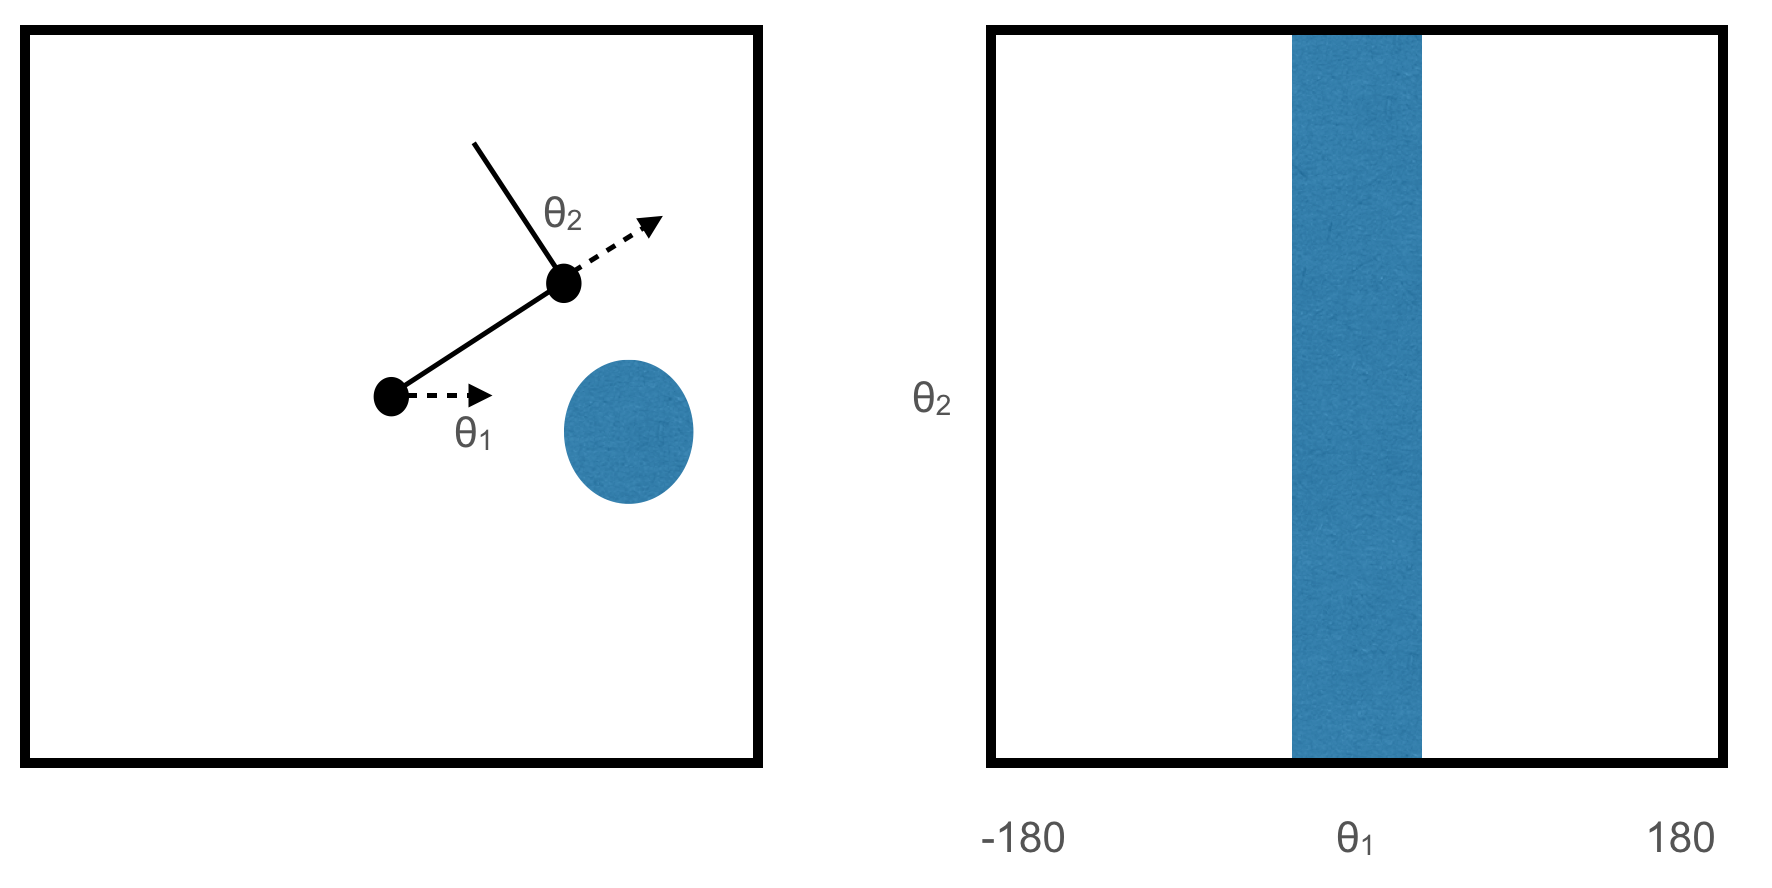
\includegraphics[scale=0.4, center]{figures/robotarmsolutions}
\else
  \bigskip
  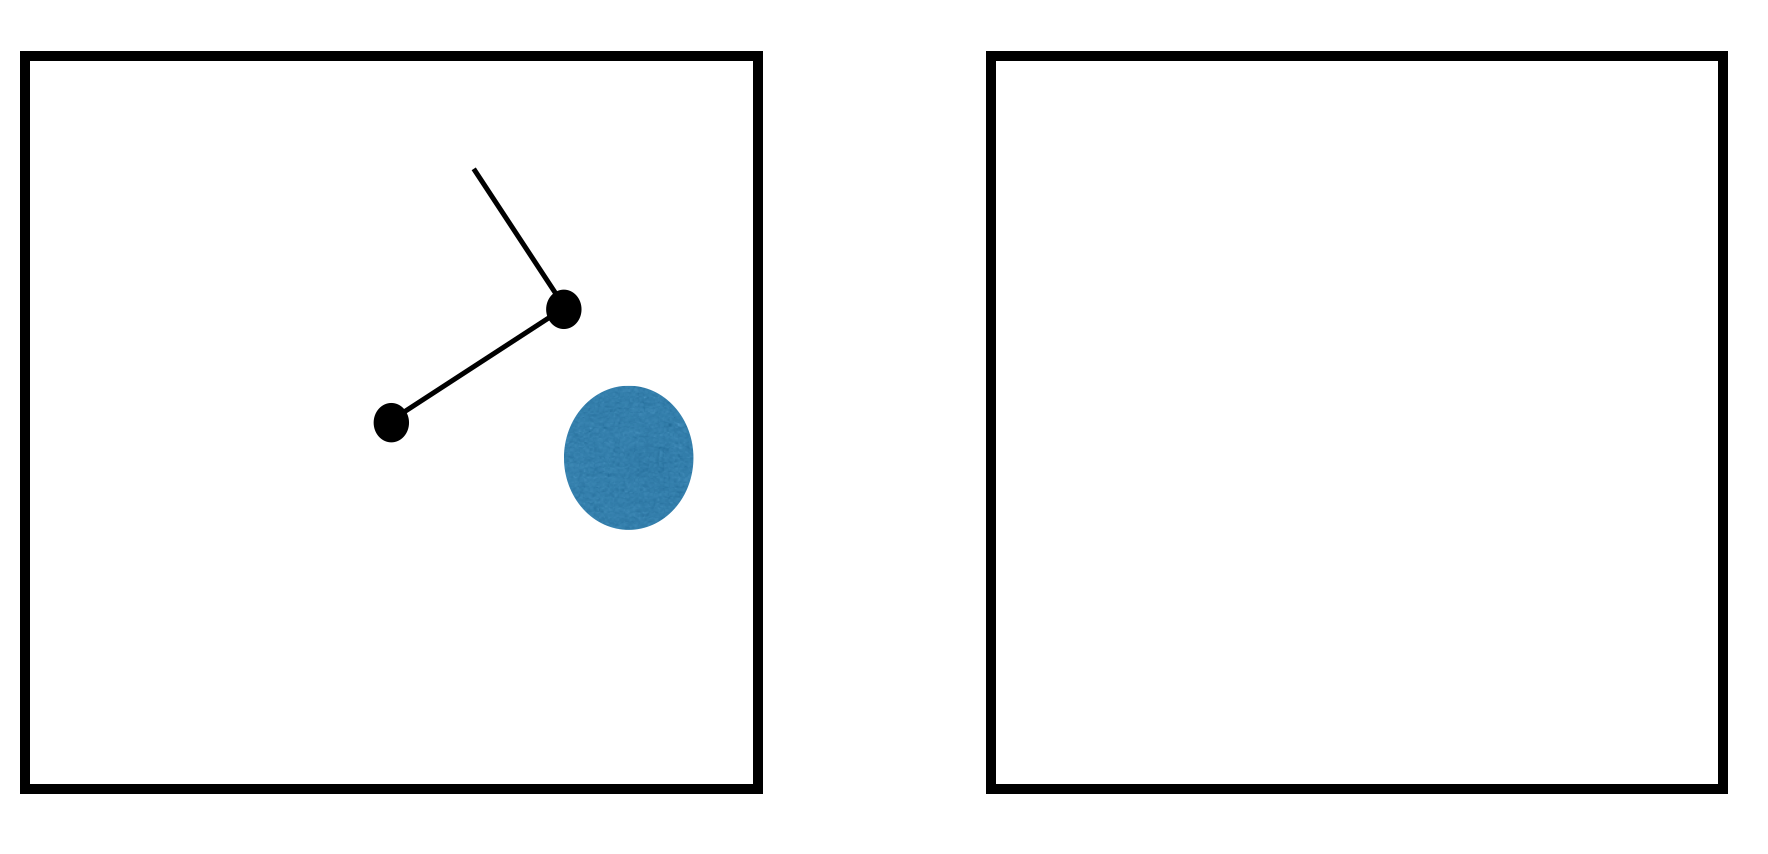
\includegraphics[scale=0.4, center]{figures/robotarm}
\fi


\newpage

{\bf{Exercise 2}}

Consider the ``elbow'' robot from above. Assume the following points
are sampled for PRM, with the given start and goal nodes. Create a graph
for the PRM using the 3-nearest neighbors approach,
and find the shortest path from $s$ to $g$.

\ifsol
  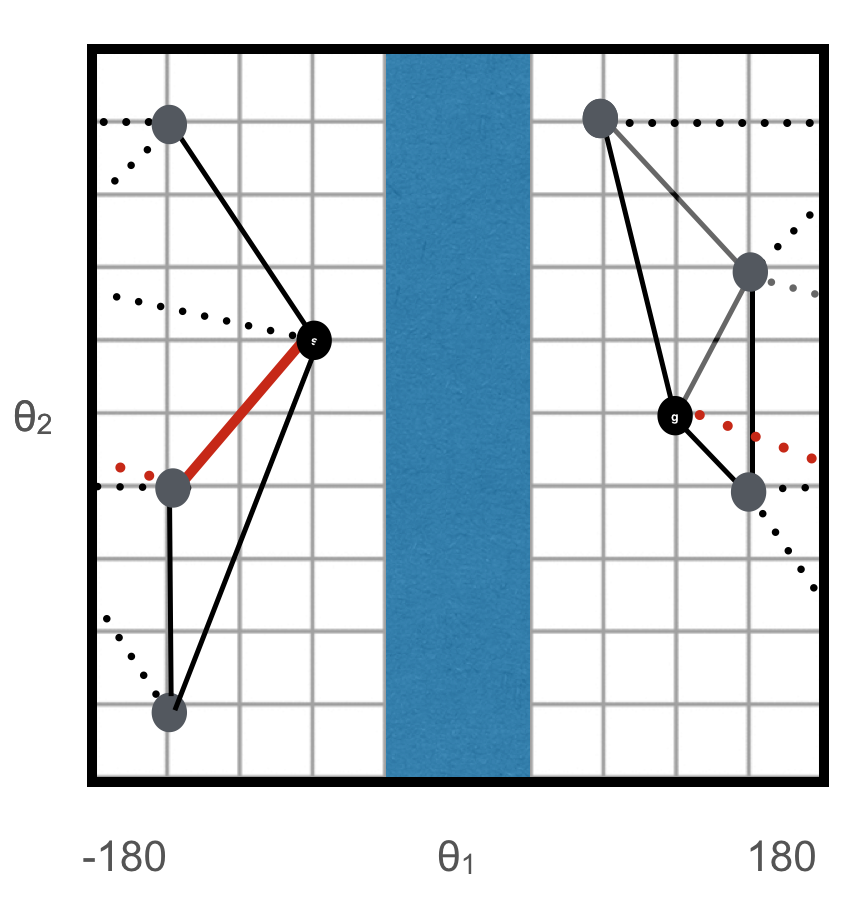
\includegraphics[scale=0.65, center]{figures/finalfinalfinalfinalprmsoln}
\else
  \bigskip
  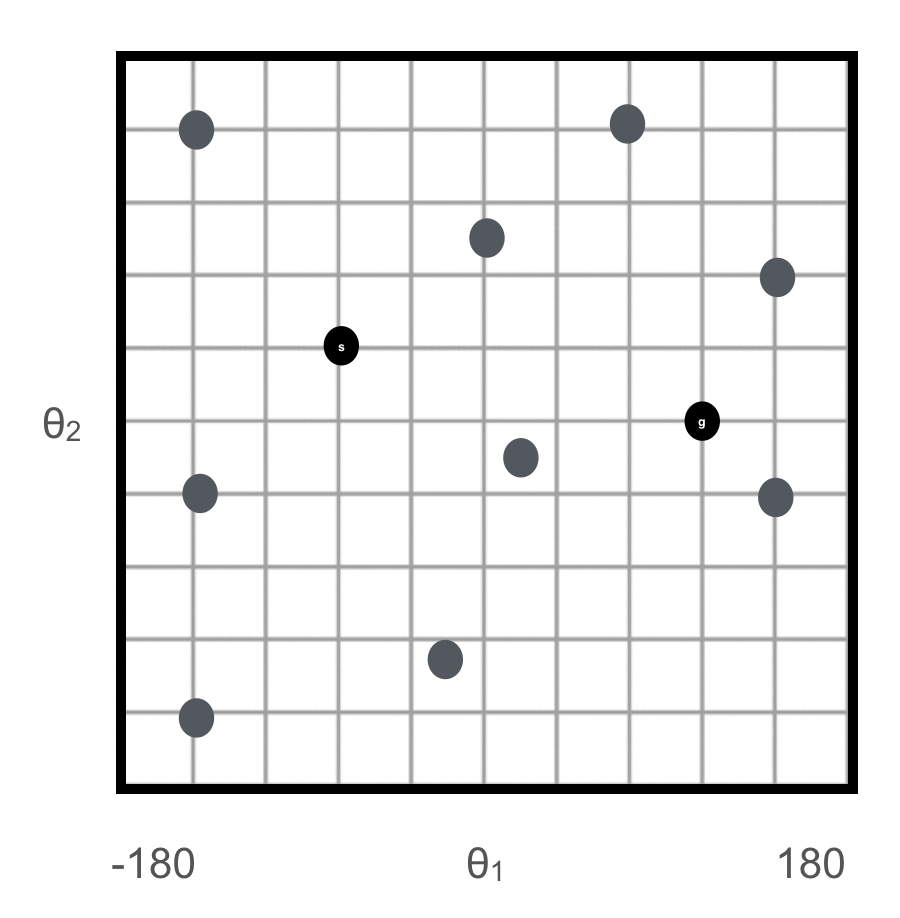
\includegraphics[scale=0.75, center]{figures/finalfinalfinalprmproblem}
\fi

\newpage


{\bf{Exercise 3}}

Assume the following figure shows the first $7$ states sampled, in order, through RRT and RRT*. Trace out the tree formed by the first $7$ steps of RRT, and RRT*. For RRT* assume a radius of $2.99$ for checking better paths and a maximum extension distance of 2.25.

\ifsol
    \begin{figure}[ht]
    \centering
    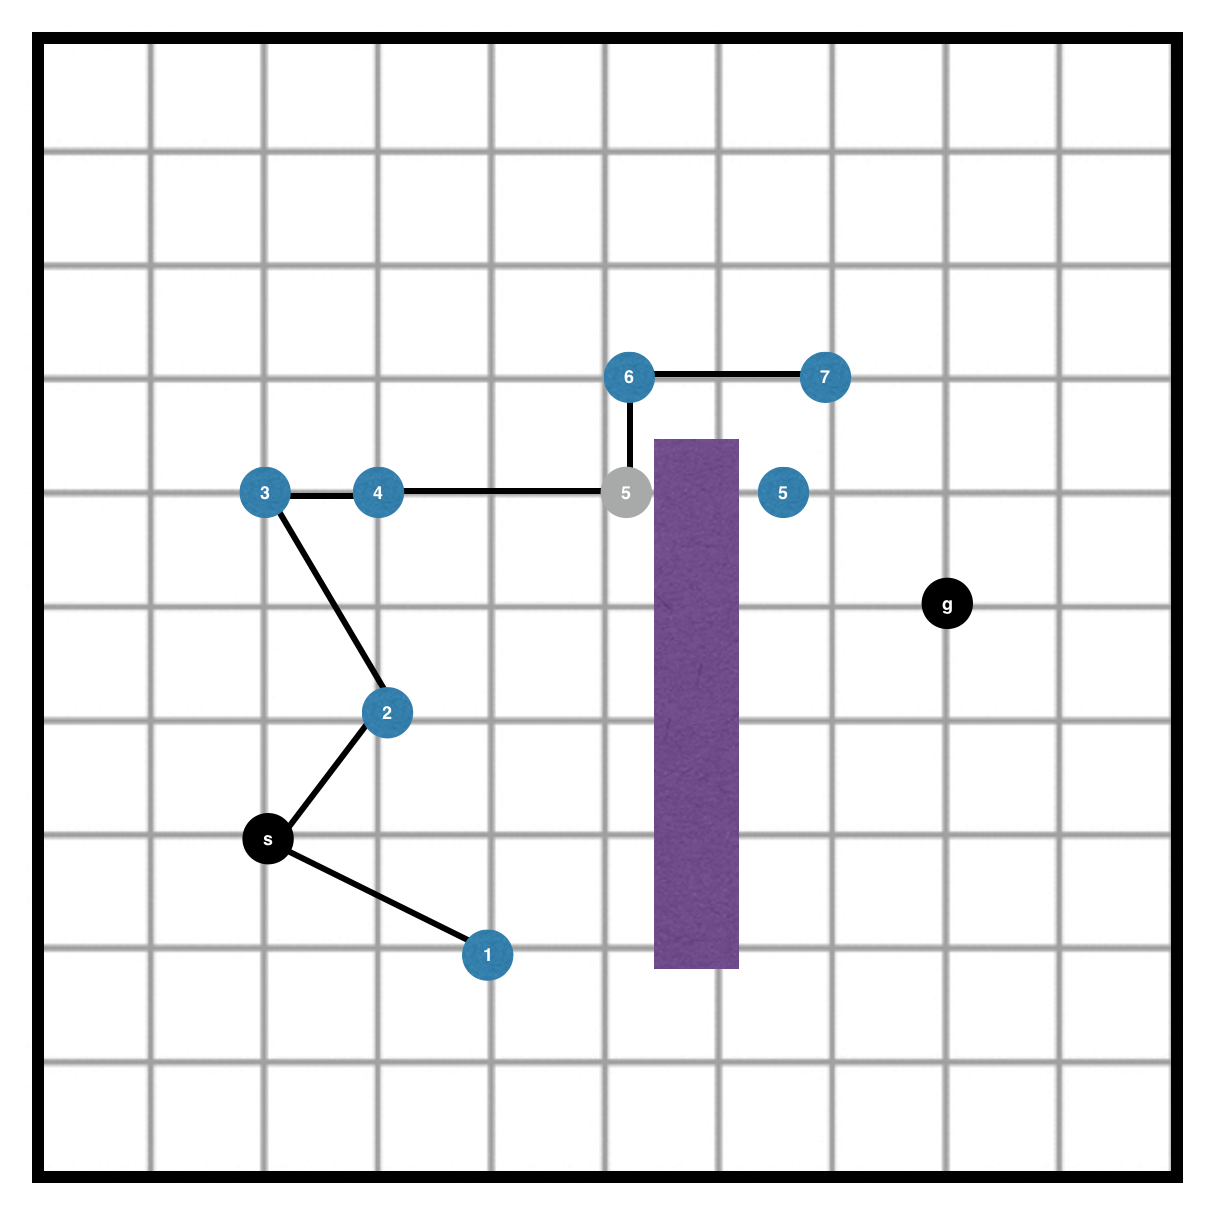
\includegraphics[scale=0.35]{figures/finalfinalfinalrrtsoln}
    \caption{RRT}
    \end{figure}
    
    \begin{figure}[ht]
    \centering
    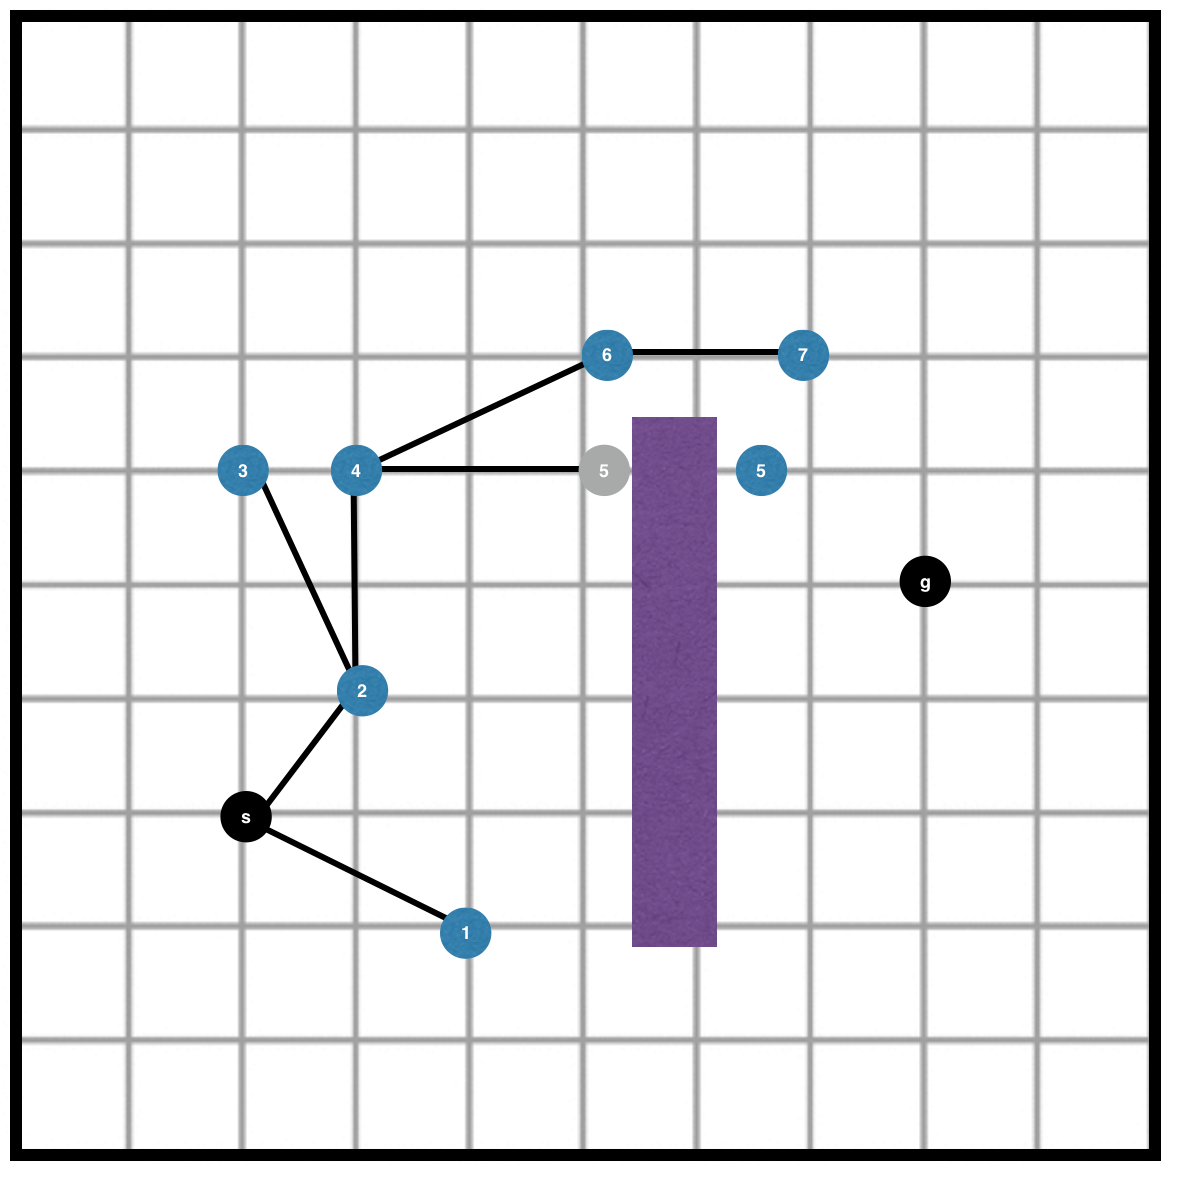
\includegraphics[scale=0.35]{figures/finalfinalfinalrrtstarsoln}
    \caption{RRT*}
    \end{figure}
\else
    \bigskip
    \begin{figure}[ht]
    \centering
    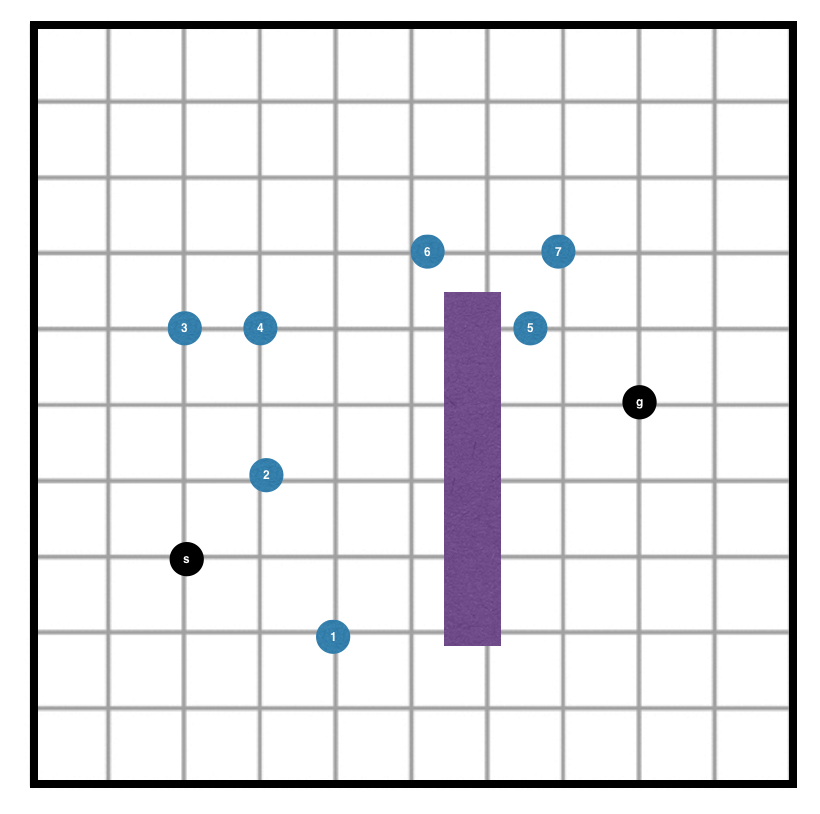
\includegraphics[scale=0.5]{figures/finalfinalrrtproblem}
    \caption{RRT}
    \end{figure}
    
    \begin{figure}[ht]
    \centering
    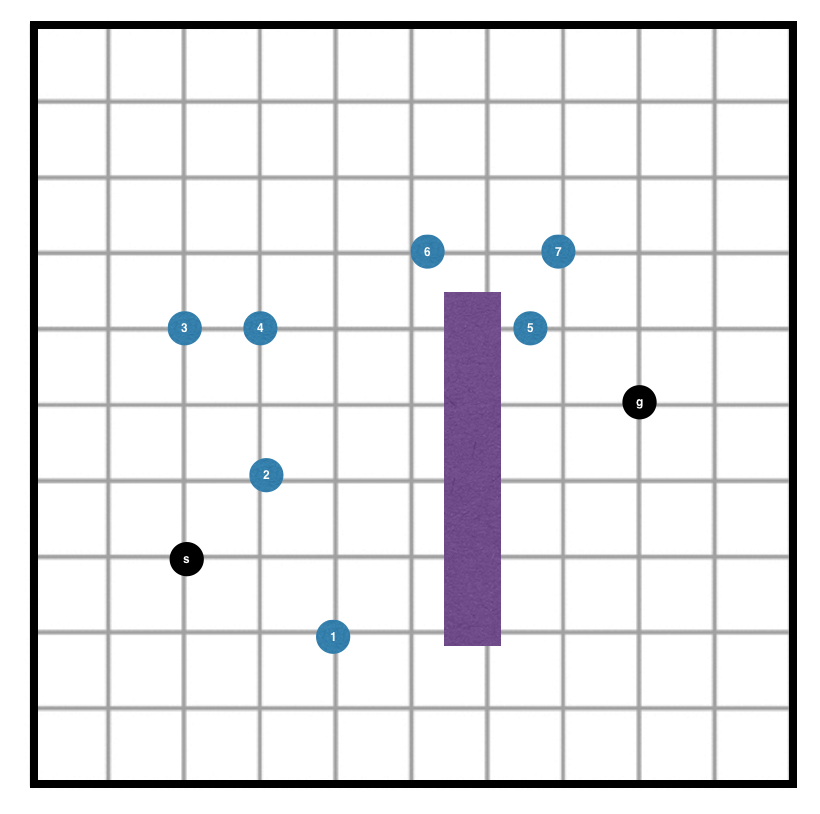
\includegraphics[scale=0.5]{figures/finalfinalrrtproblem}
    \caption{RRT*}
    \end{figure}
\fi


\clearpage
\end{document}
